\chapter{Sprecyzowanie typu aplikacji generowanych przez narzędzie} \label{chap:generated_app_type}

Po zebraniu założeń dotyczących rdzenia narzędzia generującego aplikacje, nadszedł czas na wybór typu aplikacji, które będą generowane przez narzędzie.



%=======
\section{Wybór typu aplikacji}
%=======

Narzędzie powinno generować taki typ aplikacji, aby można było w~pełni zbadać jego użyteczność i~ocenić, na ile eliminuje ono duplikację.
Aby było to możliwe, narzędzie powinno generować aplikacje, w~których występuje dużo potencjalnych miejsc występowania duplikacji.

Wymaganie to spełniają aplikacje o~architekturze wielowarstwowej (ang. \emph{multi-tier architecture, n-tier architecture}~\cite{ntier}).


\subsection{Architektura wielowarstwowa}

Architektura wielowarstwowa to taka, w~której ogólne obszary przetwarzania danych w~aplikacji są fizycznie rozdzielone pomiędzy osobne komponenty.
Współpraca pomiędzy tymi komponentami jest zorganizowana w~taki sposób, że komponent $A$ może korzystać z~funkcjonalności komponentu $B$ tylko wtedy, gdy komponent $B$ należy do warstwy logicznie umiejscowionej nie wyżej niż warstwa, do której należy komponent $A$.

Przykładem, a jednocześnie najpopularniejszą realizacją tej architektury jest architektura trójwarstwowa (ang. \emph{three-tier architecture}), która wprowadza podział aplikcji na trzy warstwy:

\begin{enumerate}
 \item Warstwa prezentacji (ang. \emph{Presentation Layer}) - odpowiada za komunikację z~użytkownikiem aplikacji (np. poprzez interfejs graficzny) lub innymi systemami (np. poprzez usługi sieciowe); jest to warstwa logicznie najwyższa;
 \item Warstwa logiki biznesowej (ang. \emph{Business Logic Layer, BLL}) - odpowiada za przetwarzanie danych zgodnie z~wymaganiami funkcjonalnymi aplikacji;
 \item Warstwa dostępu do danych (ang. \emph{Data Access Layer, DAL}) - udostępnia mechanizmy odczytu i~zapisu danych składowanych przez aplikację (np. w~pamięci lub w~bazie danych); jest to warstwa logicznie najniższa.
\end{enumerate}

Współpracę pomiędzy warstwami architektury trójwarstwowej przedstawia diagram zamieszczony na rysunku~\ref{fig:three_tier}.

\begin{figure}[!ht]
 \begin{center}
  \scalebox{0.7}
  {
   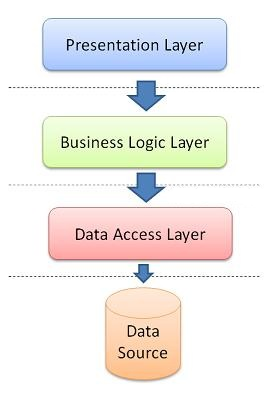
\includegraphics{figures/generated_app_type/three_tier.png}
  }
 \end{center}
 \caption{Współpraca pomiędzy warstwami architektury trójwarstwowej~\cite{three_tier}.}
 \label{fig:three_tier}
\end{figure}


W~takiej architekturze elementy dziedziny aplikacji często mają swoje odwzorowanie w~każdej z~warstw, na przykład:

\begin{itemize}
 \item jako obiekty modelu w~warstwie dostępu do danych;
 \item jako obiekty biznesowe (ang. \emph{business object})~\cite{business_object} w~warstwie logiki biznesowej;
 \item jako modele widoków (ang. \emph{view model})~\cite{view_model} interfejsu użytkownika lub obiekty tranportu danych (ang. \emph{Data Transfer Object, DTO})~\cite{dto} usług sieciowych w~warstwie prezentacji.
\end{itemize}

To sprawia, że aplikacja o~architekturze wielowarstwowej jest narażona na powszechne występowanie duplikacji wiedzy na temat dziedziny aplikacji, a~tym samym dobrze nadaje się jako typ aplikacji generowanych przez narzędzie.



%=======
\section{CQRS}
%=======

Przypadkiem szczególnym architektury wielowarstwowej jest architektura CQRS (\emph{Command Query Responsibility Segregation})~\cite{cqrs}.
Zakłada ona podział wszystkich działań w~aplikacji na dwa rodzaje:

\begin{itemize}
 \item zapytanie (ang. \emph{query}) - działanie polegające na pobraniu danych z~bazy danych (lub innego źródła danych);
 \item komenda (ang. \emph{command}) - działanie polegające na modyfikacji danych w~bazie danych.
\end{itemize}

Działania te w~architekturze CQRS są rozłączne.
Ich wykonywaniem zajmują się dwa osobne modele danych aplikacji:

\begin{itemize}
 \item model zapytań (ang. \emph{Query Model}) - model przeznaczony do odczytu danych;
 \item model komend (ang. \emph{Command Model}) - model przeznaczony do modyfikacji danych.
\end{itemize}


Koncepcyjny schemat tej architektury przedstawia rysunek~\ref{fig:cqrs}.

\begin{figure}[!ht]
 \begin{center}
  \scalebox{0.5}
  {
   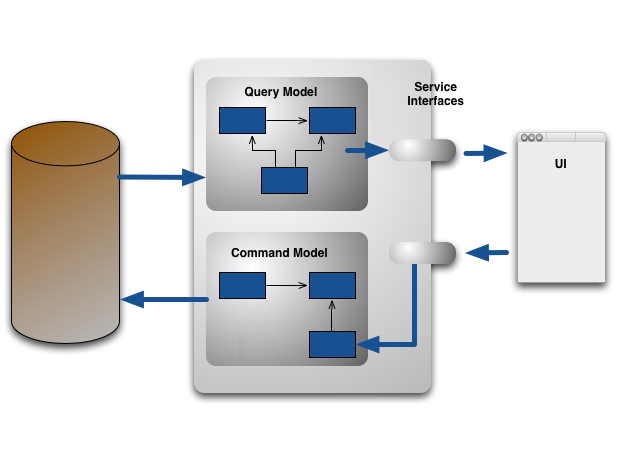
\includegraphics{figures/generated_app_type/cqrs.png}
  }
 \end{center}
 \caption{Schemat architektury CQRS~\cite{cqrs}.}
 \label{fig:cqrs}
\end{figure}


Podział odpowiedzialności pomiędzy komponenty przedstawia się następująco:

\begin{itemize}
 \item model zapytań zajmuje się odczytywaniem danych z~bazy danych;
 \item odpowiedzialnością modelu komend jest realizacja logiki biznesowej aplikacji, w~tym weryfikacja poprawności danych, aktualizacja danych w~bazie danych itd.;
 \item warstwa prezentacji (\emph{UI}):
  \begin{itemize}
   \item wyświetla dane pobrane z~modelu zapytań za pośrednictwem interfejsów (\emph{Service Interfaces}),
   \item przekazuje - w~postaci komend - akcje wykonywane przez użytkownika do modelu komend.
  \end{itemize}
\end{itemize}

Celem wprowadzenia takiego podziału jest



Specyficzną cechą aplikacji aprtych o~tę architekturę jest to, że operują one na modelach o~wysokim stopniu denormalizacji, co wiąże się z~powszechnie występującą duplikacją metadanych.


\begin{itemize}
 \item opisać CQRS
 \item że często idzie w parze z Event Sourcing
\end{itemize}

Wybór tej architektury wniesie problemy do rozwiązania podczas implementacji generatora:

\begin{itemize}
 \item gdzie w CQRS zdefiniowana jest dziedzina (encje) aplikacji? Model do odczytywania nie zawiera przecież encji, a tylko widoki.
 \item model "read" i model "write" częściowo na siebie zachodzą (lub nawet "read" zawiera "write"). Jak uniknąć duplikacji metadanych?
\end{itemize}

\begin{itemize}
 \item wybrać typ aplikacji
 \item dlaczego CQRS
  \item bo zdenormalizowana dziedzina
 \item że webowa (bo bardzo dzisiaj popularny typ)
\end{itemize}



%=======
\section{Event sourcing}
%=======

\begin{itemize}
 \item opisać Event Sourcing
 \item że całość dobrze idzie w parze z NoSQL
\end{itemize}



%=======
\section{NoSQL}
%=======

\begin{itemize}
 \item opisać NoSQL
  \begin{itemize}
   \item opisać rodzaje baz NoSQL
   \item wybrać bazę NoSQL i dlaczego Cassandra
  \end{itemize}
\end{itemize}



%=======
\section{Cassandra}
%=======

opisać Cassandrę
